
\section{Introduction}
The Reduced Area Medical Rectangular Oncological Device (RAMROD) is a proposed proton synchrotron for treatment of cancer patients.  The device will deliver up to 2
Gray per second (\gs) to a 1 $mm^3$ tumor area.  The beam will originate in a 50 mA ion source, will be accelerated through a radio frequency quadropole (RFQ) and 
a drift tube linear accelerator (DTL) up to 7~\mev of energy. The beam will be injected into the synchrotron lattice, and accelerated to 250~\mev.  The sextopole 
magnet will be ramped to create the specific beam shape needed for a slow extraction over a few seconds.  During the extraction, the betatron tune is adjusted
to push more central protons into the 3rd order resonance arms for extraction.  In this way a high extraction efficiency can be achieved.  The extraction is 
performed by placing an electrostatic septum set to 100 kV/cm at a point where a single arm of the 3rd order resonance will intersect the field region.  These
particles will receive a ``kick'' and begin moving away from the central beam.  Further down the lattice there will be a thin magnetic septum to further bend the extracted
particles into the downstream beam pipe and toward the treatment area.  Using this method a constant dose can be delivered over several seconds to an area.  The depth of 
proton penetration can be adjusted by either placing a suitable moderating material before the patient, or reducing the energy of the extracted beam.  The beam may be 
scanned over a small area during the several seconds in order to deliver dose in a grid to different parts of the tumor.  

\section{Lattice}

\begin{figure}[h]
  \begin{center}
    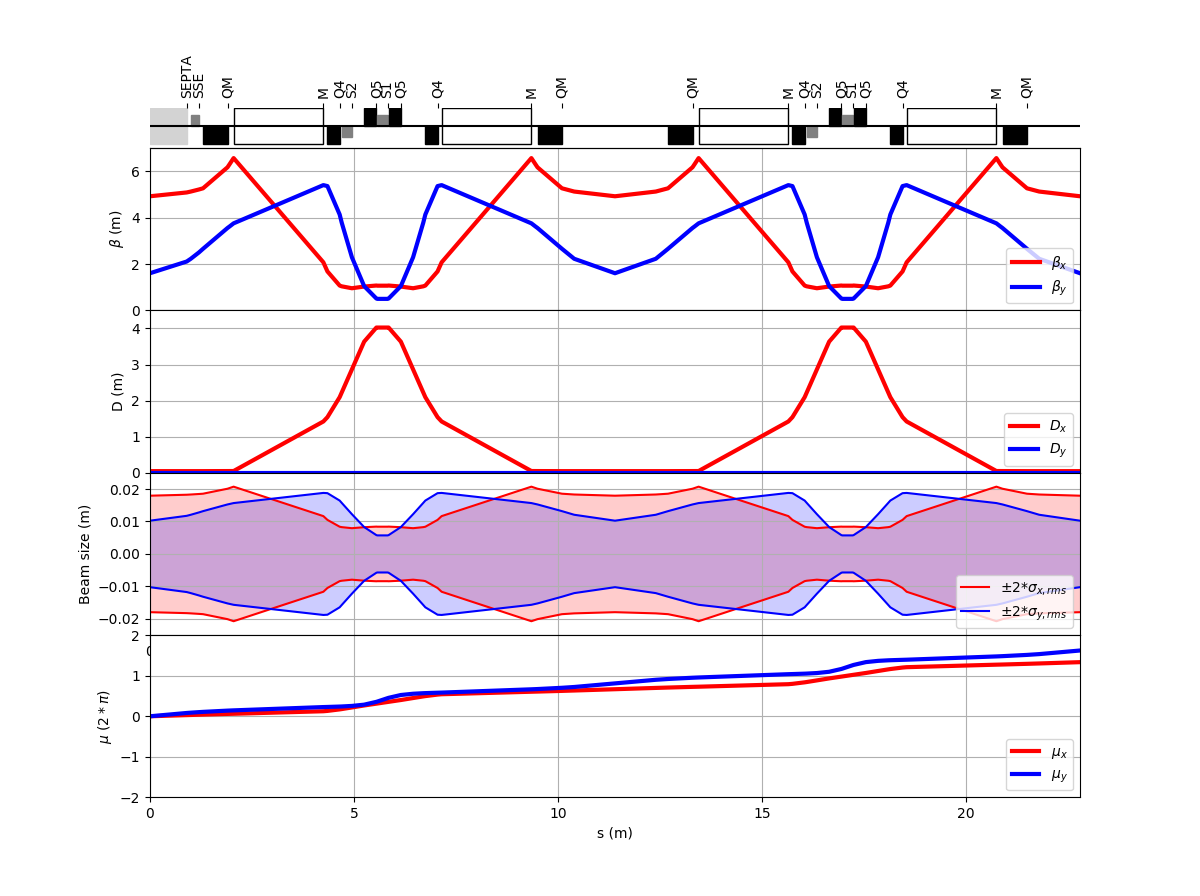
\includegraphics[width=0.45\textwidth]{twiss_33.png}
    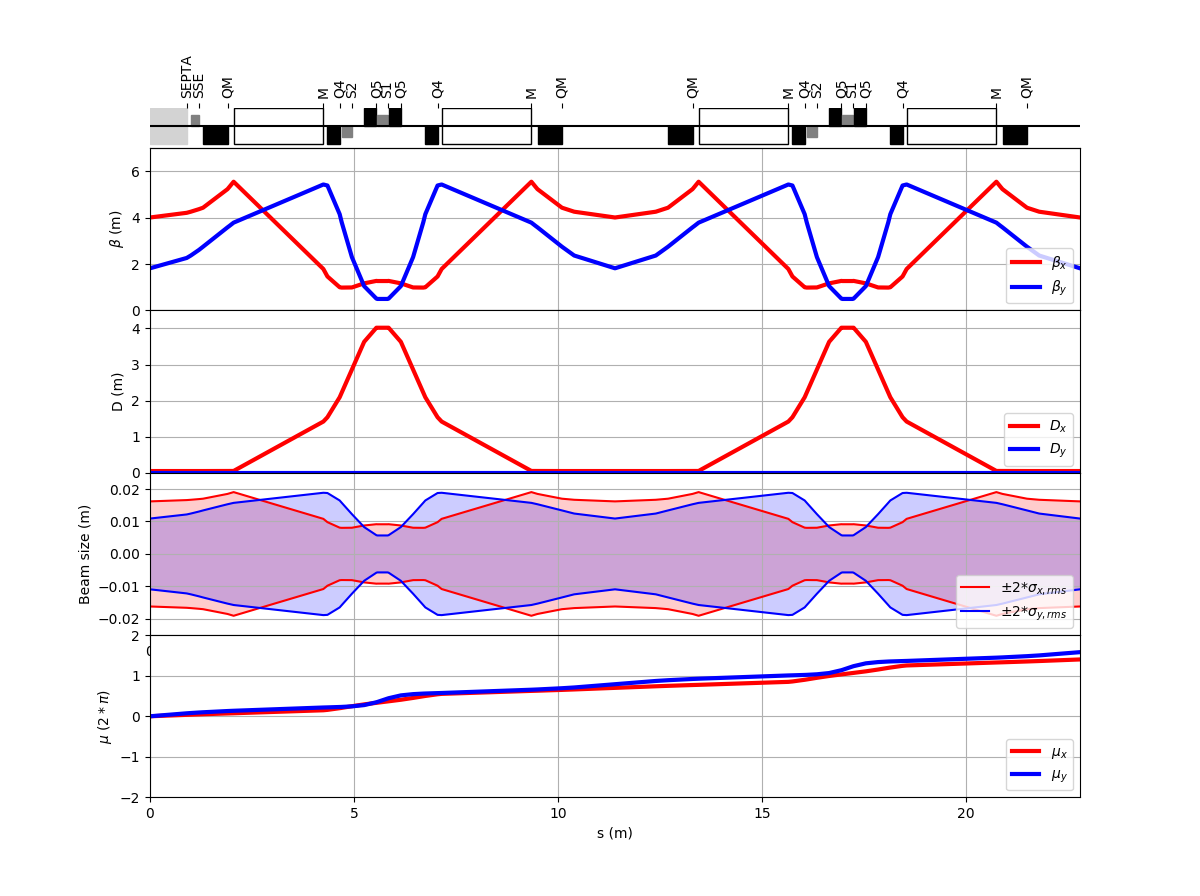
\includegraphics[width=0.45\textwidth]{twiss_40.png}
    \caption{Lattice}
  \end{center}
  \label{fig:lat}
\end{figure}


\section{Source, Injection and Extraction}


